\documentclass[12pt]{article}


\usepackage{amssymb}
\usepackage{amsmath}
\usepackage{fullpage}
\usepackage{epsfig}
\usepackage{epstopdf}
\everymath{\displaystyle}



\begin{document}

\begin{center}
\underline{\LARGE{Chapter 4.4 Practice Problems}}
\end{center}

\noindent EXPECTED SKILLS:

\begin{itemize}

\item Be able to find the absolute maxima and minima of a function, and where they occur, over a given interval.

\item Be able to state and apply the Extreme Value Theorem, where appropriate.

\end{itemize}

\noindent PRACTICE PROBLEMS:

\medskip

\begin{enumerate}

\item  Consider the graph of $y=f(x)$, shown below. For each of the following, compute the absolute maximum and absolute minimum values of $f(x)$ on the given interval, if they exist.  (Make reasonable assumptions about the behavior of the function outside of the shown interval.)

\begin{center}
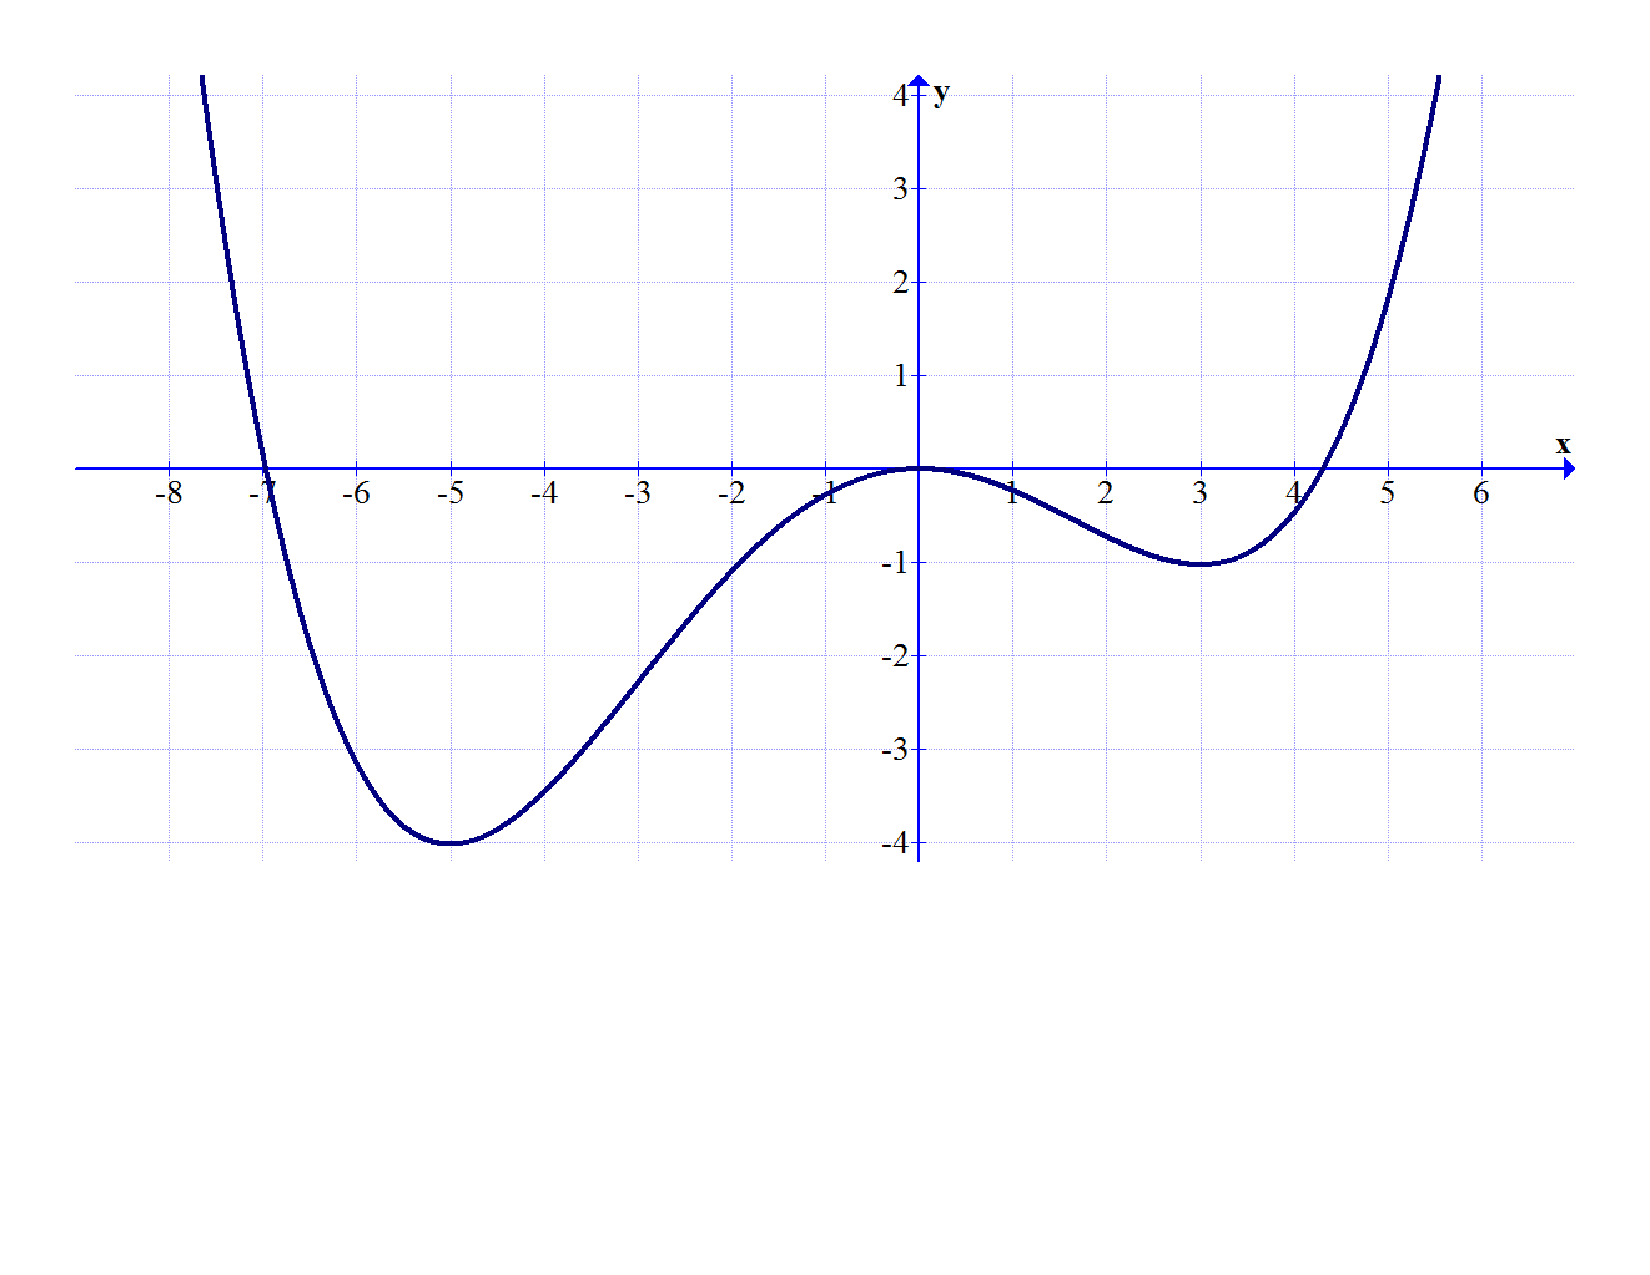
\includegraphics[scale=0.5]{graph.pdf}
\end{center}

\begin{enumerate}

\item $(-\infty,\infty)$

\includegraphics[scale=0.5]{start.pdf}
{{No absolute maximum; Absolute minimum of $-4$ when $x=-5$}}
\includegraphics[scale=0.5]{end.pdf}


\item $[-7,5]$

\includegraphics[scale=0.5]{start.pdf}
{{Absolute maximum of 2 when $x=5$; Absolute minimum of $-4$ when $x=-5$}}
\includegraphics[scale=0.5]{end.pdf}


\item $[-6,-2]$

\includegraphics[scale=0.5]{start.pdf}
{{Absolute maximum of $-1$ when $x=-2$; Absolute minimum of $-4$ when $x=-5$}}
\includegraphics[scale=0.5]{end.pdf}


\item $[-7.5,-6]$

\includegraphics[scale=0.5]{start.pdf}
{{Absolute maximum of $3$ when $x=-7.5$; Absolute minimum of $-3$ when $x=6$}}
\includegraphics[scale=0.5]{end.pdf}


\item $(-4,1)$

\includegraphics[scale=0.5]{start.pdf}
{{Absolute maximum of 0 when $x=0$; No absolute minimum}}
\includegraphics[scale=0.5]{end.pdf}


\end{enumerate}

\item Sketch the graph of a continuous function, $y=f(x)$, which has all of the following properties:

\begin{itemize}

\item $f(x)$ has a domain of $[1,7]$

\item $f(x)$ has an absolute maximum of 6 when $x=2$ and an absolute minumum of $-1$ when $x=5$.

\item $f^{\prime \prime}(x)>0$ for all $x$ in the domain of $f(x)$, with the exception of $x=2$ where $f^{\prime \prime}(x)$ DNE.

\end{itemize}

\includegraphics[scale=0.5]{start.pdf}
{{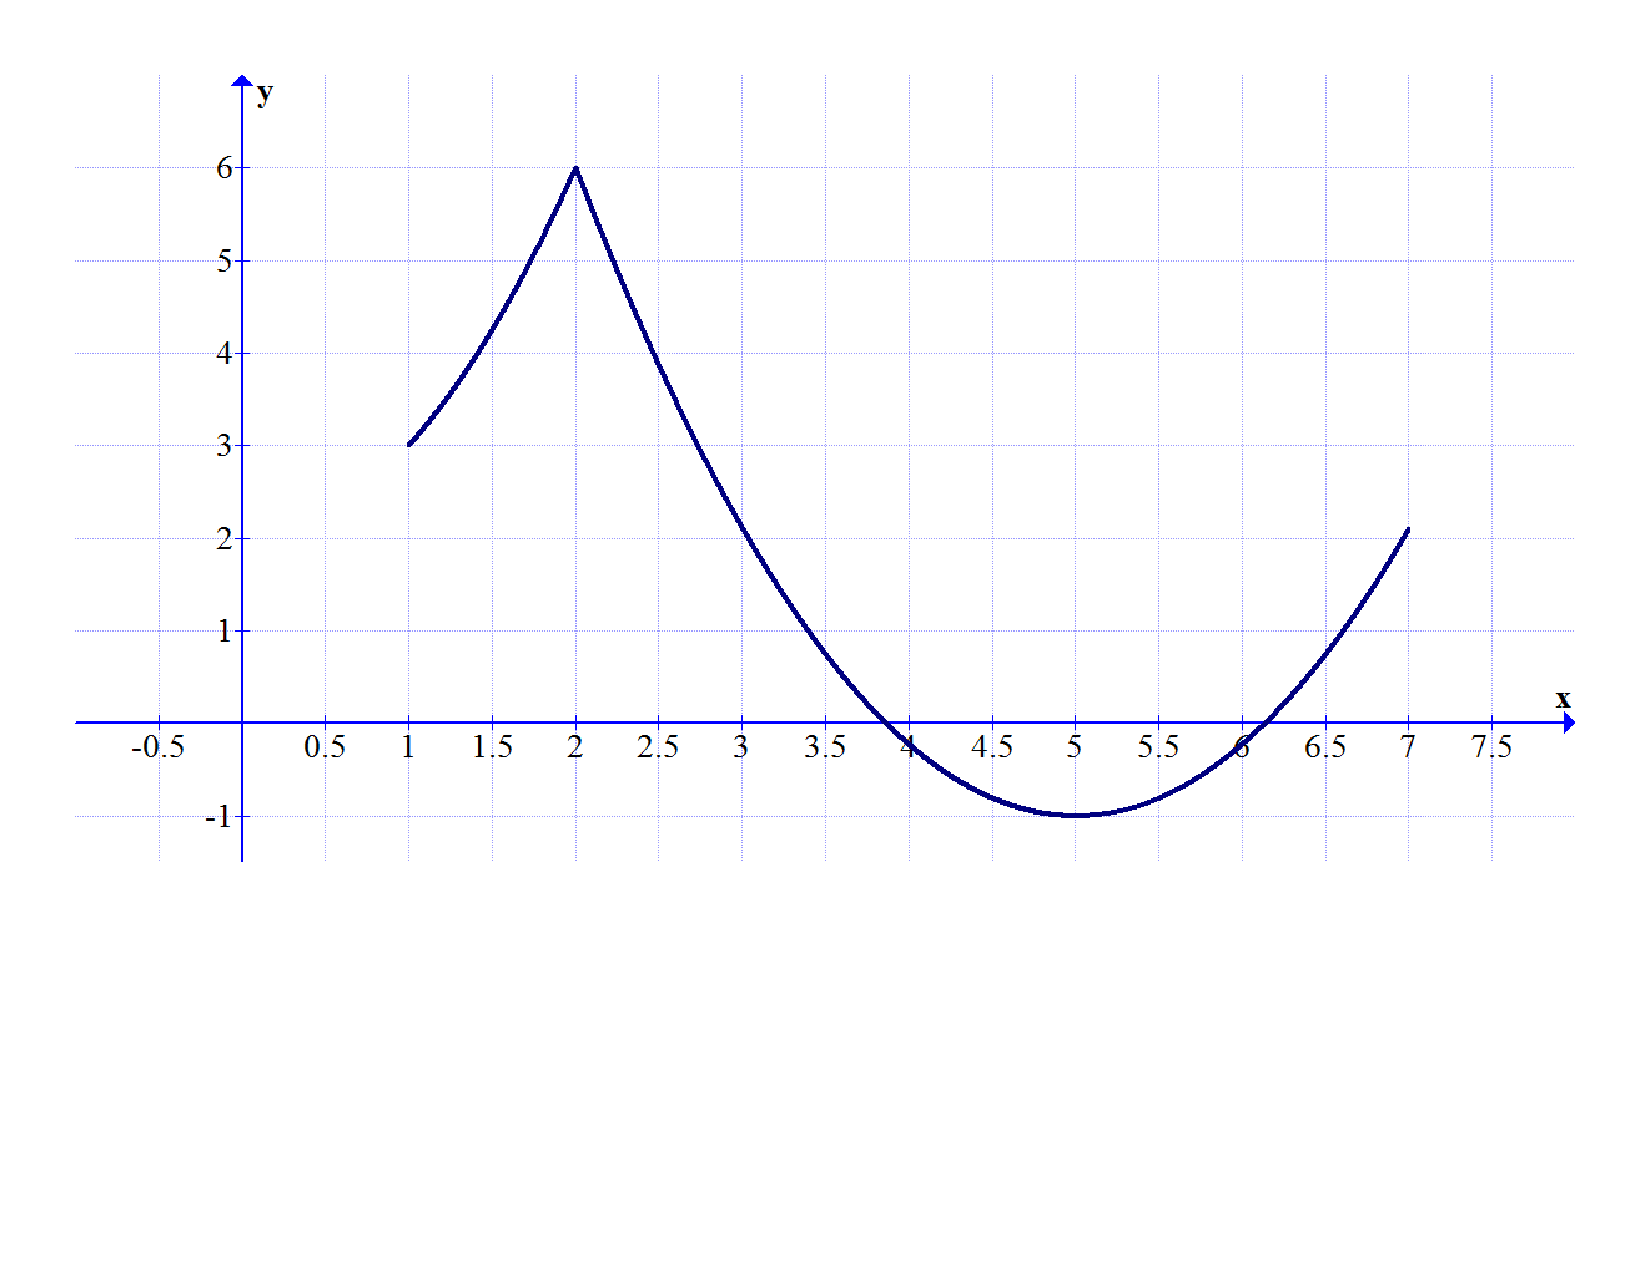
\includegraphics[scale=0.3]{graph2.pdf}}}
\includegraphics[scale=0.5]{end.pdf}


\end{enumerate}

\noindent {\bf For each of the following, find the absolute maximum and minimum values of $f(x)$ on the given interval.}

\begin{enumerate}
\setcounter{enumi}{2}

\item $f(x) = x^2+3x-4$ on $[-3,3]$. 

\includegraphics[scale=0.5]{start.pdf}
{{absolute maximum of $14$ when $x=3$; absolute minimum of $\frac{-25}{4}$ when $x=\frac{3}{2}$}}
\includegraphics[scale=0.5]{end.pdf}


\item $f(x) =(2x+1)^3$ on $[-1,4]$. 

\includegraphics[scale=0.5]{start.pdf}
{{absolute maximum of $729$ of $x=4$; absolute minimum of $-1$ when $x=-1$}}
\includegraphics[scale=0.5]{end.pdf}


\item $f(x) = \frac{x-3}{(x-4)^2}$ on $[-4,1]$. 

\includegraphics[scale=0.5]{start.pdf}
{{absolute minimum of $-\frac{2}{9}$ when $x=1$, absolute maximum of $-\frac{7}{64}$ when $x=-4$}}
\includegraphics[scale=0.5]{end.pdf}


\item $f(x) = \cos{x}-\sin{x}$ on $[-\pi,\pi]$. 

\includegraphics[scale=0.5]{start.pdf}
{{absolute maximum of $\sqrt{2}$ when $x=-\frac{\pi}{4}$, absolute minimum of $-\sqrt{2}$ when $x=\frac{3\pi}{4}$}}
\includegraphics[scale=0.5]{end.pdf}


\item $f(x) = \sqrt{1-x^2}$ on $[-1,1]$ 

\includegraphics[scale=0.5]{start.pdf}
{{absolute minimum of 0 when $x=-1$ and when $x=1$; absolute maximum of 1 when $x=0$}}
\includegraphics[scale=0.5]{end.pdf}


\item $f(x) = |x-3|$ on $[-5,5]$ 

\includegraphics[scale=0.5]{start.pdf}
{{absolute minimum of 0 when $x=3$, absolute maximum of 8 when $x=-5$}}
\includegraphics[scale=0.5]{end.pdf}


\item $f(x) = x^{\frac{1}{3}}(x-5)^2$ on $[1,10]$ 

\includegraphics[scale=0.5]{start.pdf}
{{absolute minimum of 0 when $x=5$, absolute maximum of $25 \cdot \sqrt[3]{10}$ when $x=10$}}
\includegraphics[scale=0.5]{end.pdf}


\item $f(x) = \tan{x}+\sin{x}$ on $\left[-\frac{\pi}{4}, \frac{\pi}{4}\right]$ 

\includegraphics[scale=0.5]{start.pdf}
{{\begin{tabular}{ll}
absolute minimum of $-1-\frac{\sqrt{2}}{2}$ when $x=\frac{\pi}{4}$\\
\\
absolute maximum of $1+\frac{\sqrt{2}}{2}$ when $x=-\frac{\pi}{4}$
\end{tabular}
}}
\includegraphics[scale=0.5]{end.pdf}


\item $f(x) = 3x^2-4x+9$ on $(-\infty, \infty)$ 

\includegraphics[scale=0.5]{start.pdf}
{{no absolute maximum, absolute minimum of $\frac{23}{3}$ when $x=\frac{3}{2}$}}
\includegraphics[scale=0.5]{end.pdf}


\item $f(x) = -x^2+5x-10$ on $(-\infty, \infty)$ 

\includegraphics[scale=0.5]{start.pdf}
{{no absolute minimum, absolute maximum at $-\frac{15}{4}$ when $x=\frac{5}{2}$}}
\includegraphics[scale=0.5]{end.pdf}


\item $f(x) = \frac{x-2}{x+5}$ on $(-\infty, \infty)$ 

\includegraphics[scale=0.5]{start.pdf}
{{none}}
\includegraphics[scale=0.5]{end.pdf}


\item $f(x) = x^2e^{-2x}$ on $(-\infty, \infty)$  

\includegraphics[scale=0.5]{start.pdf}
{{no absolute maximum, absolute minimum of 0 when $x=0$ }}
\includegraphics[scale=0.5]{end.pdf}


\end{enumerate}

\end{document}